% !TeX root = Par_paket.tex
%!TEX program = lualatex

\documentclass[12pt]{exam} %addpoints, togs bort för att testa andra poäng
\usepackage[swedish]{babel}
%\usepackage[utf8]{inputenc}
\usepackage[T1]{fontenc}
\usepackage{mathtools}
\usepackage{amssymb}
\usepackage{amsthm}
\usepackage{kmath}
\usepackage{kerkis}
\usepackage{systeme}
\usepackage{graphicx}
\usepackage[parfill]{parskip}
\usepackage[a4paper,left=1cm, right=1cm,top=1.5cm, bottom=2cm]{geometry}
\usepackage{siunitx}
\usepackage{enumitem}
\usepackage{multicol}
\usepackage[sharp]{easylist}
\usepackage{pgfplots}
\pgfplotsset{compat=1.8}
\usepgfplotslibrary{statistics}
\usepackage{tkz-euclide}
\usetikzlibrary{colorbrewer}
\usetikzlibrary{arrows}
\usepackage{caption}
\usepackage{subcaption}
\usepackage{float}
\usepackage{xcolor}
\usepackage{setspace}
\usepackage{datatool}
%\DTLloaddb{koder}{test.txt}
\usepackage[sc]{titlesec}
\usepackage{tabularray}
\usepackage[strict]{changepage}
\usepackage{wrapfig}
\usepackage{emoji}
\setemojifont{TwemojiMozilla}
\usepackage{caption}


\usepackage[most]{tcolorbox} 
\definecolor{block-gray}{gray}{0.95}


\newtcolorbox{zitat}[2][]{%
    colback=block-gray,
    grow to right by=-10mm,
    grow to left by=-10mm, 
    boxrule=0pt,
    boxsep=0pt,
    breakable,
    enhanced jigsaw,
    borderline west={4pt}{0pt}{gray},
    title={#2\par},
    colbacktitle={block-gray},
    coltitle={black},
    fonttitle={\large\bfseries},
    attach title to upper={},
    #1,
    text width=4.5cm,
}


\renewcommand\qedsymbol{$\blacksquare$} % namn till olika text miljöer
\theoremstyle{plain}% default
\newtheorem{thm}{Sats}
\newtheorem{lem}[thm]{Lemma}
\newtheorem{prop}[thm]{Proposition}
\newtheorem*{cor}{Korollarium}


\theoremstyle{definition}
\newtheorem{defn}{Definition}
\newtheorem{exmp}{Exempel}
\newtheorem{upg}[exmp]{Uppgift}

\theoremstyle{remark}
\newtheorem*{rem}{Tips}
\newtheorem*{note}{Anmärkning}

\everymath{\displaystyle}


\colorgrids % gör att svarsrutnäten är ljusgrå
\colorfillwithdottedlines
\setlength{\gridlinewidth}{0.7pt}
\definecolor{GridColor}{gray}{0.9}
%\pointsinrightmargin 
\setlength{\rightpointsmargin}{2cm}
%\pointformat{\fbox{\phantom{\themarginpoints }/\themarginpoints}}
\marginpointname{}

% Svenska namn till poänglista
%\pointpoints{Poäng}{Poäng}
%\bonuspointpoints{Bonuspoäng}{Bonuspoäng}
\pointpoints{}{}
\bonuspointpoints{}{}
\totalformat{Uppgift \thequestion: \totalpoints{} poäng}
\hqword{Uppgift:}
\hpgword{Sida:}
\hpword{Poäng:}
\hsword{Resultat:}
\htword{Total}

%För att skriva ut fråge namn och inga siffror
\qformat{\sc\thequestiontitle\dotfill\thepoints 
\vrule depth 1em width 0pt
} 

\newcommand{\mild}{\emoji{hot-pepper}}
\newcommand{\medel}{\emoji{hot-pepper}\emoji{hot-pepper}}
\newcommand{\het}{\emoji{hot-pepper}\emoji{hot-pepper}\emoji{hot-pepper}}

\firstpageheader{\bfseries Inlämning utkast:\draft , Slutlig:\final}{}{\large\bfseries Namn:\enspace\makebox[2in]{\hrulefill}}
\runningheader{}{}{\oddeven{\large\bfseries Namn:\enspace\makebox[2in]{\hrulefill}}{}}% skriver bara ut namn på varanan sida. Dvs en gång per papper vid dubbelsidig utrskrift.

\firstpagefooter{\class}{\thepage\ (\numpages)}{}
\runningfooter{\class}{\thepage\ (\numpages)}{}


\newcommand{\ovning}{
\usepackage{draftwatermark}
\SetWatermarkColor{red!10}
\SetWatermarkScale{1}
\SetWatermarkText{Övning}     %Watermark text
%\usepackage{pgfmorepages}
%\pgfmorepagesloadextralayouts
%\pgfpagesuselayout{repeated 2-up}[a4paper,landscape]
}


% For an exam, single spacing is most appropriate
\singlespacing
% \onehalfspacing
% \doublespacing


%%%% Inställningar för provet %%%%

% Kommentera bort om det inte ska stå övning på provet
%\ovning 

\newcommand{\class}{Ma2c}
\newcommand{\term}{HT 24}
\newcommand{\nummer}{1}
\newcommand{\draft}{17/5}
\newcommand{\final}{19/5}
%\newcommand{\timelimit}{15 minuter} 
%\newcommand{\hjalp}{Chromebook med geogebra / Räknare, Formelsamling} % I minuter
\pgfmathdeclarefunction{gauss}{2}{%
  \pgfmathparse{1/(#2*sqrt(2*pi))*exp(-((x-#1)^2)/(2*#2^2))}%
}
\sisetup{locale = DE}

\begin{document}
\begin{center}
{\Large \textsc{PAR Problem nr.}\nummer}\\[0.3cm]
\end{center}

\fbox{\fbox{\parbox{\textwidth}{{
\noindent \centering PAR Processen\\
Skriv ett utkast \hspace{0.3cm} Reflektera \hspace{1.1cm} Feedback \hspace{1.3cm} Förbättra \hspace{1.2cm} Lämna in \phantom{te}\\
\includegraphics*[width=15cm]{img/par_prosess.png}\\}
\phantom{testtesttset}(Hemma) \hspace{1.4cm} (Hemma) \hspace{0.5cm} (Fredags lektionen) \hspace{0.3cm} (Hemma) \hspace{0.5cm} (Tisdags lektionen) }}}
\smallskip \vspace{0.5cm}

    


% -------------------------------------------------------------

%Here, the questions begin
\begin{questions}
%\setlength\itemsep{2\baselineskip}

\titledquestion{Glasspaketet}
De hungriga ungdomarna Asta, Bea och Cesar ska dela på ett glasspaket. Diskussionen uppstår då hur
paketet ska delas rättvist. På kanten finns en markering som de förstår är mitten av paketet (E). Asta
drar då två sträckor utifrån den mittpunkten (AE) samt paketets hörn (BD) (de streckade sträckorna på bilden) och skär sedan av paketet i
skärningspunkten (F) och påstår att hon tagit exakt en tredjedel, den bit som utgörs av fyrhörningen ABHG.
Stämmer det?
\begin{figure}[H]
    \centering
    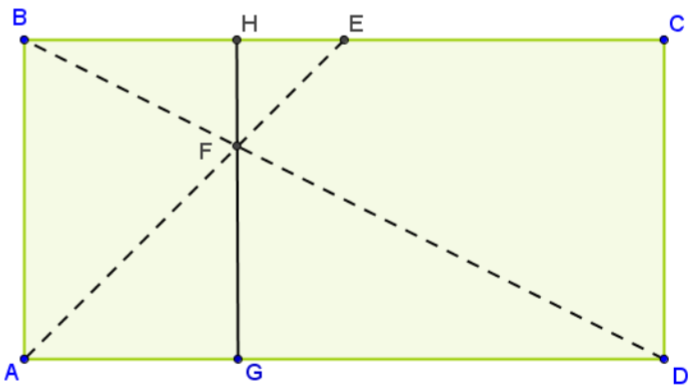
\includegraphics[width=0.5\linewidth]{img/Glasspaket.png}
    \caption{Ett glasspaket.}
\end{figure} %Ändra till den uppgift som ska byggas


%-------------------------------------------------------------------
%Här kommer svars områden och sånt
\newpage
\begin{center}
  Feedback av:\enspace\makebox[2in]{\hrulefill}\\
\end{center}

\smallskip
\noindent Styrkor \hfill Kommunikation \hfill Förslag \hrule

\begin{figure}[H]
    \centering
    
\includegraphics[width=1.5cm, page=3]{img/Bilder.pdf}
    \caption*{Lätt att följa alla steg.}
    
\includegraphics[width=1.5cm, page=2]{img/Bilder.pdf}
    \caption*{Förklarar varför,\\ inte bara vad.}
    
\includegraphics[width=1.5cm, page=1]{img/Bilder.pdf}
    \caption*{Använder namn.}
    
\includegraphics[width=1.5cm, page=5]{img/Bilder.pdf}
    \caption*{Tydliga definitioner av variabler.}
    
\includegraphics[width=1.5cm, page=6]{img/Bilder.pdf}
    \caption*{Använder diagram.}
\end{figure}

\noindent Styrkor \hfill Korrekthet \hfill Förslag \hrule
\begin{figure}[H]
  \centering
  
\includegraphics[width=1.5cm, page=8]{img/Bilder.pdf}
  \caption*{Korrekta beräkningar}
  
\includegraphics[width=1.5cm, page=9]{img/Bilder.pdf}
  \caption*{Testat olika sätt.}
  
\includegraphics[width=1.5cm, page=10]{img/Bilder.pdf}
  \caption*{Rimligt svar.}

\end{figure}
\newpage
\section*{Utkast}
\fillwithgrid{\stretch{1}}
\newpage
\fillwithgrid{\stretch{1}}
\newpage
\section*{Slutinlämning}
\fillwithgrid{\stretch{1}}
\newpage
\fillwithgrid{\stretch{1}}


\end{questions}
\end{document}
